%--------------------------------------------------------------------------------
% Master thesis 2018 Lukas Strebel
%--------------------------------------------------------------------------------

\documentclass[11pt, a4paper]{article}

%--------------------------------------------------------------------------------
% Packages
%--------------------------------------------------------------------------------
\usepackage{a4}
\usepackage[a4paper]{geometry}
\usepackage{amsfonts}
\usepackage{amsmath}
\usepackage{mathtools}
\usepackage[utf8]{inputenc}
\usepackage{fancyhdr}
\usepackage{setspace}
\usepackage[hidelinks]{hyperref}
\usepackage[htt]{hyphenat}
\usepackage{listings}
\usepackage{xcolor}
\usepackage{graphicx}
\usepackage{tcolorbox}
\usepackage{booktabs}
\usepackage{longtable}
\usepackage{pdfpages}
\usepackage{natbib}
\usepackage{subcaption}
\usepackage[linesnumbered,lined,boxed,commentsnumbered]{algorithm2e}

%--------------------------------------------------------------------------------
% Commands
%--------------------------------------------------------------------------------

% Graphics path
\graphicspath{{figure/}}

\newgeometry{left=3cm,bottom=3.0cm}
\setlength{\headheight}{14.49998pt}
\onehalfspacing

% Page Style
\pagestyle{fancy}
\renewcommand{\sectionmark}[1]{\markright{\thesection\ #1}}
\fancyhead{}

%This labels the page
\rhead{\thepage}
\lhead{\nouppercase{\rightmark}}
\fancyfoot{}

% Tables
\newcommand{\ra}[1]{\renewcommand{\arraystretch}{#1}}

% partial derivatives
\newcommand{\pdv}[2]{\frac{\partial #1}{\partial #2}}

% Python listing
% Default fixed font does not support bold face
\DeclareFixedFont{\ttb}{T1}{txtt}{bx}{n}{\small} % for bold
\DeclareFixedFont{\ttm}{T1}{txtt}{m}{n}{\small}  % for normal

% Custom colors
\usepackage{color}
\definecolor{deepblue}{rgb}{0,0,0.5}
\definecolor{deepred}{rgb}{0.6,0,0}
\definecolor{deepgreen}{rgb}{0,0.5,0}

\usepackage{listings}

% Python style for highlighting
\lstset{
language=Python,
basicstyle=\small\ttm,
breaklines=true,
otherkeywords={self},             % Add keywords here
keywordstyle=\ttb\color{deepblue},
emph={MyClass,__init__},          % Custom highlighting
emphstyle=\ttb\color{deepred},    % Custom highlighting style
stringstyle=\color{deepgreen},
frame=single,                         % Any extra options here
showstringspaces=false            % 
}

\newcommand\numberfont{\normalfont\footnotesize\color{Numbers}}
\newcommand\basicfont{\small\ttfamily}

% Floor sign
\DeclarePairedDelimiter{\floor}{\lfloor}{\rfloor}

%--------------------------------------------------------------------------------
% Title page
%--------------------------------------------------------------------------------
\newcommand{\mytitlepage}
{
    \newpage
    \thispagestyle{empty}
    \begin{spacing}{1}
    \begin{center}
        {\large Master thesis}\\
        \vspace{\stretch{1}}\doublespacing
        {\LARGE\bf Automatic domain decomposition for HPC stencil codes in heterogeneous systems}\\
        \vspace{\stretch{1}}
        {\large\bf Lukas Strebel}\\
        {lstrebel@ethz.ch}\\
        \vspace{\stretch{4}}
        {\small Supervisor}\\
        Prof. Thomas Schulthess \\
        Dr. Lucas Benedicic \\
        \vspace{1.5\baselineskip}
        Swiss National Supercomputing Centre (CSCS)\\
        Swiss Federal Institute of Technology Zürich (ETH)\\
        \vspace{\stretch{2}}
        {\large \monthyeardate\today}\\
        \vspace{\stretch{2}}
        \begin{tabular*}{\linewidth}{l@{\extracolsep{\fill}}r}
            
\includegraphics[height=13mm]{CSCS_logo.png} & 
            
\includegraphics[height=13mm]{ETHlogo.png}
        \end{tabular*}
    \end{center}
    \end{spacing}
    \clearpage
    \thispagestyle{empty}
    \setcounter{page}{1}
    \null
    %\newpage
}
%---------------------------------------------------------------------
% Document body
%---------------------------------------------------------------------
\begin{document}

% === Title ===
\pagenumbering{roman}
\mytitlepage

% === Abstract ===
\addcontentsline{toc}{section}{\protect\numberline{}{Abstract}}
\markright{Abstract}
\section*{Abstract}


\section*{Acknowledgements}

I would like to thank CSCS and ETH for providing the opportunity to take on this thesis project.
I would also like to thank Prof. Thomas Schulthess for supervising my Master thesis.

Also thanks to my other supervisor Lucas Benedicic for guiding me throughout the whole thesis.

Additionally, thanks to Felipe Cruz for helping with various problems.

As well as a special thanks to Stefano Ubbiali for not only providing the reference codes used throughout the thesis, but also for helping with any questions I had.



%% Start ToC on right page
\clearpage
\thispagestyle{empty}
\null
\newpage

% === Table of contents ===
\newpage
\tableofcontents
\addtocontents{toc}{\vspace{.5\baselineskip}}

% label pages in arabic
\pagenumbering{arabic}
\setcounter{page}{6}

\cleardoublepage

% === Chapters ===
\section{Introduction}
\subsection{Problem statement}
The overarching problem addressed in this thesis is the decomposition of the computational domain for stencil based simulations.
Domain decomposition is necessary to distribute and balance the computational load among distributed processing units.
Additionally, including heterogeneous processing units adds further complications to the domain decomposition problem.

Solutions to the domain decomposition problem should be automatic, i.e. require a minimal amount of manual input.
Automating domain decomposition helps separating concerns between domain scientists and computer scientists.

Therefore, the thesis focuses on the creation of an automatic domain decomposition library addressing these problems.

\subsection{Background}
Most scientific or engineering codes that model and simulate natural phenomena require more computational resources than a single processing unit can provide.
Distributed systems, such as high performance clusters, are a common way to provide the necessary resources for complex simulations.
However, porting such codes from their usually serial form to codes that run in parallel on distributed systems creates several challenges.
These challenges are generally outside the scope of the domain specific developers.

Decomposing the computational domain and distributing it to the processing units is one of these challenges.

\subsubsection{Distributed heterogeneous systems}
Distributed systems have been used for decades in high performance computing (HPC) to compute simulations for various scientific fields.
A more recent development is the introduction of accelerator devices e.g. graphics processing units (GPU) to the nodes in HPC clusters.
These accelerator devices bring enormous computational power with their large number of cores for throughput-critical computations.
But their architecture is different compared to CPUs for latency-critical applications.

Therefore, some HPC systems have a hybrid configuration of CPUs and GPUs to combine the advantages of both architectures.
However, this also means that nodes in HPC clusters no longer have homogeneous processing units, which makes the distribution of the computational domain ever more complex.
\citet{mittal2015survey} provide a more detailed description of the evolution and motivation behind heterogeneous computing.

\subsubsection{Stencil codes}
Domain decomposition is used in various type of simulations.
This thesis focuses on domain decomposition for stencil codes.

Stencil codes are a family of codes commonly used in various scientific computing applications.
The name "stencil codes" refers to computations using a fixed pattern of values from points on a mesh.

These fixed patterns often originate from explicit finite difference approximations on structured meshes.
Structured meshes guarantee that every point in the mesh, except points on the boundary, has the same number of neighboring points.
Explicit finite difference approximations use the values on the mesh at a given point in time to compute the values for the next small time step.
Finite difference approximations are one common way to solve partial differential equations (PDEs).
Numerous scientific fields - such as fluid dynamics or climate dynamics - model the natural phenomena of their studies as PDEs.

A single time step in a stencil code consists of iterating through every point on the mesh according to the fixed pattern, gathering values from other points, and using these values to compute the value for the next time step.
Simulations of complex natural phenomena usually require very fine spatial and temporal resolutions as well as computations involving multiple different quantities on every grid point.
Therefore, even theoretically simple stencil codes are in practice frequently more intricate.

Complex stencil codes usually require their large mesh to be decomposed into computational sub-domains for each processing unit to be solved in a reasonable amount of time.
Therefore, domain decomposition is an important part of stencil codes.

\subsubsection{Domain decomposition / graph partitioning}
Domain decomposition can be seen as a specific form of load balancing for codes in which the load is roughly equal for each point in a domain.
Stencil codes fulfill this characteristic.

The sub-domains that result from domain decomposition for stencil codes need to synchronize the values across their boundaries to be consistent.
This synchronization requires communication between the different processing units.

The quality of a given domain decomposition is determined by the balance of computational load among all processors and the reduction of communication among different processors.

A common way to model and solve domain decomposition is through graph partitioning.
When using this strategy, the elements of the discrete domain are represented by the vertices of a graph, with edges representing the connections between neighboring elements.
The sum of all values on the edges between two sub-domains is called the edge cut.
The edge cut in this model represents the total amount of communication between the two sub-domains.

Therefore, graph partitioning algorithms that use a cost function to minimize such an edge cut, while maintaining an approximate uniformity of sub-domain size, provide domain decompositions that minimize the communication cost.

\subsection{Related works}
\label{sec:relwork}
In literature, the process of creating sub-domains from a larger domain is referred to by different names: domain decomposition, static mapping, (graph) partitioning, topology mapping, or sometimes more general as a form of load balancing.

Domain decomposition is used to account for different computational load imbalances in various simulations.
Common sources for such imbalances are irregular grids (e.g. finite element method), task-based applications, or heterogeneous communication costs.
In \citet{saxena2015architecture} it is stated that heterogeneous architectures have not received as much attention as a source of imbalance.
Nevertheless, heterogeneous architectures are a source of imbalance even for simulations that do not have any other source of imbalance.

However, even for different sources of imbalance, most often the problem is modeled as a graph, and a graph partitioning algorithm is used to solve for a domain decomposition.

In the general case, graph partitioning has been proven to be NP-complete (\citet{feldmann2015balanced}).
However, relaxing the constraint to roughly equal instead of exactly equal partitions allows various different heuristics to generate a sub-optimal solution in reasonable time.

A general overview and comparison between different graph partitioning algorithms can be found in \citet{karypis1998fast}.
Specifically, Table 9 illustrates different criteria for useful graph partitioning and how each algorithm ranks in them.
Even though this paper is a few years old, both of the most common graph partitioning libraries, METIS \footnote{\href{http://glaros.dtc.umn.edu/gkhome/views/metis}{http://glaros.dtc.umn.edu/gkhome/views/metis}} and SCOTCH \footnote{\href{https://gforge.inria.fr/projects/SCOTCH/}{https://gforge.inria.fr/projects/SCOTCH/}}, are based on the basic algorithms described in the paper.

While conceptually very similar the algorithms in these libraries differ in their mathematical description and their modeling approach.

\subsubsection{SCOTCH library}
The SCOTCH library models the problem as a set of two graphs:
a valuated, undirected source graph $S(V, E)$ representing the parallel processes (vertices) and communication channels (edges). And a not-valuated target graph $T(V, E)$ representing the topology of the target machine.
The target graph is not valuated because it assumes an homogeneous architecture.

To solve the graph partitioning on these two graphs, the SCOTCH library employs a dual recursive bipartitioning algorithm.
This algorithm is formulated by \citet{pellegrini1994static} in the following way:

The goal of a mapping is then defined as:
$\varphi : V\left(S\right) \rightarrow V\left(T\right)$ such that $\varphi\left(v_s\right) = v_t $ if $v_s$ is mapped onto processor $v_t$.
\\
And $\psi : E\left(S\right) \rightarrow E\left(T\right)$ such that $\psi\left(e_S\right) = \left\{ e_T^1, e_T^2, \dots, e_T^n \right\}$ with $\left| \psi\left(e_S\right) \right|$ as the number of edges in the target graph that are used.
\\
With these definitions, the cost function to be minimized is defined as the edge cut function $f_c$:
\begin{equation}
f_c\left(\varphi, \psi \right) = \sum_{e_s \in \text{cut} \left(E\left(S\right)\right)} \left(c\left(e_S\right) \cdot \left| \psi\left(e_S\right) \right| \right)
\end{equation}
where $c\left(e_S\right)$ is the value of the edge (i.e. the communication cost) and $\text{cut} \left(E\left(S\right)\right)$ contains all edges belonging to the two subsets of the bipartition for which the cost function is computed.

\subsubsection{METIS library}
The older METIS library was developed on the basis of a multilevel bipartitioning algorithm.
In their model, a single valuated, undirected source graph is partitioned, assuming that the target architecture has uniform cost for any communication between two processes.
However, the graph partitioning algorithm in the METIS library has been expanded, as explained in \citet{karypis1998multilevel}, to allow multiple constraints to be balanced.

\subsection{Source graph generation for stencil codes}
\label{sec:intro_source_graph}
For graph partitioning to be used for domain decomposition, a source graph representing the domain is required.

Simple one and two dimensional stencils are often either visualized as points connected with lines or written in matrix form. For example the well known stencil used in the computation of the Laplace equation can be expressed as
\begin{bmatrix}
& 1 &  \\
1 & -4 & 1 \\
& 1 & \\ 
\end{bmatrix}
, which is equivalent to writing the formula as $u_{i+1, j} + u_{i-1, j} + u_{i, j+1} +u_{i, j-1} - 4 u_{i, j}$.

The matrix form also illustrates the communication pattern needed by the stencil.
The position in the middle of the matrix represents the grid point itself.
The other non-zero entries in the matrix represent the other grid points needed in the computation.

The computational cost can be approximated by the number of non-zero entries in the matrix e.g. the Laplace stencil requires 4 additions and one multiplication with a scalar constant.

A source graph to partition a given domain could be built by creating a vertex in the source graph for every grid point in the domain.
In such a source graph, each vertex would have edges based on the communication patterns and a vertex weight based computational cost approximations of a stencil as previously described.
However, even for simple stencils, like the one used in the Laplace equation, it becomes impractical to partition such a built source graph for meshes with several millions of elements due to the size of such a source graph.

Thus we will investigate models and methods to achieve the generation of a practical source graph to partition the domain.

\subsection{Context}
Domain decomposition is not the only concern that separates scientific models from well performing HPC code.

Complex scientific codes, like numerical weather prediction and climate simulation models, have grown over years to multiple hundred thousands lines of code written by a large community of scientific developers.
Maintaining such large codes for the ever-changing HPC environment is challenging.

The GridTools library provides a domain specific language (DSL) designed to reduce this effort for stencil codes.
The main method of the GridTools DSL is to separate the concerns of the scientific model developers (domain experts) from the concerns of the computer scientists (HPC experts).
Separation is accomplished by letting the domain experts use the DSL in their model development process without the need to think about performance.
At the same time, computer scientist no longer need to understand the complete details of the model but instead can focus on optimizing the core computations used in stencil codes for different programming models and architectures as separate back-end of the GridTools DSL.

The GridTools DSL is written in C++, while domain scientist are often more familiar with higher level languages or simple Fortran as a language close to the mathematical formulations of their models.
An additional DSL for Python (GT4Py) aims to overcome this programming language barrier for domain scientist.
GT4Py adds an additional abstraction layer on top of the GridTools DSL so that domain scientists can use the simple and expressive Python syntax for model development without losing the advantages of the low-level optimizations of the GridTools back-end.

Within this context, the focus of this thesis is on the automation of the domain decomposition.
The resulting automatic domain decomposition library will be part of the larger effort to separate HPC concerns from scientific modeling concerns.

\subsection{Implementation and libraries}
The focus of this thesis is the implementation of an automatic domain decomposition library to solve the problems described in the previous sections.
The next few sections will describe some implementation aspects and existing libraries that will be used.

\subsubsection{Implementation details}
The implementation language will be Python.
Python provides simple and expressive syntax and is increasingly used in the scientific community.
Also, in the context of GT4Py, Python is the natural choice for the automatic domain decomposition library.

Standard practices for software development and testing will be employed.
This includes unit tests, continuous integration (CI), version control system, code documentation, and adhering to standard style guide conventions.

\subsubsection{Communication library}
The communication between processors is a significant part of computations involving domain decomposition.
Using a high quality communication library is therefore important.
Message Passing Interface (MPI) is the leading standard for distributed systems.
The communication model of MPI matches very well with finite difference computations and has been used in various finite difference implementations.

In the context of Python, this thesis will make use of the MPI for Python (MPI4Py) library, which provides bindings for MPI in Python.
MPI4Py is open source, and as described in \cite{dalcin2005mpi} supports the most important MPI communications, namely point-to-point, as well as collective communications of general Python objects.

Furthermore MPI4Py supports one-sided MPI.
One-sided MPI is the remote memory access (RMA) communication model of MPI.
One-sided MPI allows processes to expose part of their memory to other processes, in order for them to directly write or read from this memory.
In contrast to the two-sided communication model, this allows the decoupling of data movement and process synchronization.

Since one-sided communication models are a new trend in HPC, this thesis will explore the use of one-sided MPI in the context of domain decomposition and stencil computations.

\subsubsection{Graph partitioning library}
Solving the graph partitioning problem to determine a domain decomposition is a fundamental part of the proposed work.
However, the focus of this thesis is automating the process and modeling heterogeneous systems.
Therefore the automatic domain decomposition library will use another library to solve the underlying graph partitioning problem.

The reason for building on top of existing libraries is two-fold.
Firstly, it saves time from implementing methods to solve the underlying basic graph partitioning problem.
Secondly, building on top of popular libraries can make it easier in the future to keep up to date with the latest graph partitioning methods.

As mentioned in the state of the art review section \ref{sec:relwork} the two most popular graph partitioning libraries at the moment are METIS and SCOTCH.

\subsection{Structure of the thesis}

\section{Domain decomposition}
Domain decomposition in the context of this thesis refers to the process of dividing a computational domain into smaller parts in order to run on multiple processing units.
Importantly, domain decomposition in this context is not be confused with the \textit{domain decomposition method} in mathematics and numerical analysis.
The \textit{domain decomposition method} is used to solve boundary value problems by splitting them into smaller parts.
Instead, domain decomposition in high performance computing and this thesis is the name of the process used to prepare a domain for distribution to multiple processing units.
Specifically, domain decomposition in this thesis is used for solving partial differential equations using finite difference methods on multiple processing units.

The next sections outline the general approach to domain decomposition, the specifics of the model developed and used in this thesis, an overview of the graph partitioning method, and an example for the subdivision model and graph partitioning for domain decomposition.

\subsection{General approach}
Some form of domain decomposition is necessary for any distributed computation.
The process of decomposing a domain varies widely depending on the problem that is distributed i.e. the domain.

Domain decomposition approaches overlap in some aspects with load balancing methods.
For example, many approaches for both use over-decomposition.

Over-decomposition is a two step process.
First, it means splitting the problem into more parts than needed at the end.
Then in a second step combining these smaller parts into the final decomposition.

For domain decomposition this means that there needs to be a model to describe how the domain should be split into small parts.
As well as a model for distributing the smaller parts to the final domain decomposition.
The distribution of the smaller parts to the processing units handles the load balancing aspect of domain decomposition by minimizing a set of cost factors.

For domain decomposition the two main cost factors are distributing the same number of grid points to each processing i.e. \textbf{computational cost} and minimizing the amount of communication between different processing units i.e. \textbf{communication cost}.

Given these over-decomposed domain parts and their corresponding cost factors a graph partitioning algorithm can be applied to get a balanced distribution for each processing unit.

This two step process describes the general approach to domain decomposition and is described in more detail as pseudo-code in Algorithm \ref{alg:domaindecomposition}.

To note in Algorithm \ref{alg:domaindecomposition} is that the over-decomposition method introduces one new parameter: the number of subdivisions per dimension.
This parameter is further explained in Section \ref{sec:subdivmodel}.

\begin{algorithm}[!htbp]
\basicfont
\numberfont

\SetKwProg{Fn}{Function}{}{}
\SetKwProg{Ds}{Datastructure}{}{}
\SetKwFunction{SubdivideDomain}{SubdivideDomain}
\SetKwFunction{GraphPartitioning}{GraphPartitioning}
\SetKwFunction{stores}{Stores}
\SetKwFunction{StoreSubdivisionInformation}{StoreSubdivisionInformation}
\KwIn{Computational Domain, Number of Processing Units, Stencil Information}
\KwOut{Decomposed Domain, Partitioning for each Processing Unit}
\BlankLine
\Ds{DomainSubdivision}{
\stores$\left(id, size, boundaries, gridpoints, neighbors\right)$
}
\BlankLine
\Fn{DomainDecomposition(Domain, NumProcs, StencilExtent)}{
\tcc{Step 1: Over-decompose domain and store subdivisions in adjacency list.}
\\
SubdivisionWeightedAdjacencyList, ListOfDomainSubdivisions $\leftarrow$ 
\SubdivideDomain{Domain(SizePerDim, PeriodicityPerDim), NumSubdivPerDim, StencilExtent}
\\
\tcc{Step 2: Partition subdivisions based on adjacency list.}
\\
PartitionList $\leftarrow$ \GraphPartitioning{SubdivisionWeightedAdjacencyList, NumProcs}
}
\BlankLine

\Fn{SubdivideDomain(SizePerDim, PeriodicityPerDim, NumSubdivPerDim, StencilExtent)}{
\tcc{Calculate derived information:}
\\
TotalNumberOfSubdivisions $\leftarrow$ NumSubdivPerDim
\\
SizeOfSubdivision $\leftarrow$ Domain, NumSubdivPerDim
\\
SizeOfBoundaries $\leftarrow$ SizeOfSubdivision, StencilExtent
\\
\tcc{Create adjacency list:}
\\
\ForEach{Subdivision in TotalNumberOfSubdivisions}{
    \ForEach{Direction}{
        Neighbors $\leftarrow$ HandleDomainBoundaries$\left(NumSubdivPerDim, PeriodicityPerDim\right)$
        }

    AppendToWeightedAdjacencyList $\leftarrow$ Neighbors, SizeOfSubdivision, SizeOfBoundaries
\\
    \StoreSubdivisionInformation{id, size, boundaries, gridpoints, neighbors}
}
\Return SubdivisionWeightedAdjacencyList, ListOfDomainSubdivisions
}
\BlankLine
\Fn{GraphPartitioning(SubdivisionWeightedAdjacencyList, NumProcs)}{
\If{FileOutputIsEnabled}{
WriteAdjacancyListToFile(SubdivisionWeightedAdjacencyList, FormatFlag)
}
CallGraphPartitioningLibrary(SubdivisionWeightedAdjacencyList, NumProcs)
\\
\Return Partitioning
}
\BlankLine
\caption{Pseudo-code description of the two-step process to decompose a domain.}
\label{alg:domaindecomposition}
\end{algorithm}


\subsection{Subdivision model for source graph generation}
\label{sec:subdivmodel}
As mentioned before, source graphs where every source graph node represents a single physical domain grid point would be impractical for large domains.
Therefore, any alternative has to combine some of these domain grid points into separate subdivisions even before the domain decomposition occurs.

Any model for over-decomposition of domains should be guided by a few principles described in detail in Table \ref{tab:criteria}.

\begin{table}[!htbp]
\centering
\ra{1.5}
\begin{tabular}{p{4.5cm} p{9.5cm}}
\toprule
Criteria & Explanation \\
\midrule
Uniformity and regularity.
&
One of the advantages of regular grids for finite difference is simplicity of used data structures and the performance benefits these include.
Modeled domain subdivisions should keep this simplicity as well.
\\
Clearly defined and easy to determine boundaries. 
&
The boundaries between these separate subdivisions determine what and how the partitions will communicate with each other.
Creating clear and simple boundaries is necessary to make the communication process simple and as fast as possible.
The partitioning process will add complexity to the boundary communication, therefore any complexity from the over-decomposition process should be avoided.
\\
Uniform number and direction of neighbors.
&
Even though, graph partitioning can decompose graphs with vertices of various degrees, for the simplicity and performance of the communication aspect introduced by a domain decomposition the number of neighboring subdivisions should be uniform. Subdivisions at non-periodic boundaries of the physical domain are an unavoidable exception to this criteria.
\\
Simple calculations of cost functions.
&
The overall goal of providing good domain partitions can only be achieved if the graph partitioning algorithm receives good estimates for the communication and computational cost for each subdivision.
Therefore, any subdivision model needs simple but accurate estimates for both of these cost functions.
\\
\bottomrule
\end{tabular}
\caption{Criteria for over-decomposition models used to create subdivisions of a regular domain.}
\label{tab:criteria}
\end{table}

\paragraph{The simplest method}of subdividing a regular grid is by splitting it across each dimension separately, i.e. creating a number of uniform subdivisions.
This guarantees that every subdivision has the same amount of neighbors, with the exception of sections at the boundary of the physical domain if the boundary is not periodic.
Also every subdivision has the same size and therefore distributing them equally during the graph partitioning also means distributing the grid points equally.

For this kind of subdivisions it is simple to define the interior and boundary between subdivisions, as visualized for a two-dimensional and three-dimensional example in Fig. \ref{fig:2D_subdivision} and Fig. \ref{fig:3D_subdivision} respectively.
This distinction is important for the calculations of the communication and computational cost as described in Sections \ref{sec:commcost} and \ref{sec:compcost}.

One limit to the minimal size of a subdivision in any direction is given by the corresponding stencil extent.
Meaning a stencil can not extend into multiple subdivisions, but only the direct neighbor, otherwise subdivision would have multiple neighbors in the same direction.
This should not be a problem, since usually stencils are not as large as any reasonable sized subdivision.

An additional benefit from such a simple subdivision approach is that only one more parameter has to be determined i.e. the number of subdivision per dimension.

Having more subdivisions per dimension gives the graph partitioning finer control over edge cut minimization and vertex weight balance.
However, this finer control comes at the cost of more complex boundaries.
Complex boundaries meaning boundaries where more subdivisions have to communicate with each other than for more straightforward boundaries, since more communication does not necessarily mean higher communication cost for these simple estimates.

Some of these effects this parameter choice can have on the domain decomposition are mentioned in Section \ref{sec:examplesubdivision} and shown in Fig. \ref{fig:rectangular1}.

\subsubsection{Communication cost}
\label{sec:commcost}
The communication cost between subdivisions is the main criteria being minimized in the graph partitioning algorithm.
Splitting the domain into uniform subdivisions keeps the communication cost computation simple.

The communication cost for each neighbor of the subdivision is determined by the size of the boundary between the two and the extent of the stencil in the corresponding direction.

For three dimensional domains the communication cost can therefore be computed from the following formula:
\begin{equation}
cc\left(i\right) = sds\left(\left(\floor[\Big]{\frac{i}{2}} - 1\right) \% 3 \right) \cdot sds\left(\left(\floor[\Big]{\frac{i}{2}} + 1\right) \% 3 \right) \cdot se\left(i\right) \text{ ,}
\end{equation}
where $cc\left(i\right)$ is the communication cost for side $i$.
The index $i \in \left[0, 1, 2, 3, 4, 5\right]$ is combination of side and dimension, i.e. $0$ is negative x-direction, $1$ is positive x-direction, $2$ is negative y-direction, and so on.
$sds\left(j\right)$ is the subdivision size of dimension $j \in \left[0,1,2\right]$.
Lastly $se\left(i\right)$ is the stencil extend of side and dimension $i$.
The division, rounding and modulo in the formula is simply a short version of selecting the index of the other two dimensions for the computation of the area between two subdivisions.

For example, the communication cost for the subdivision shown in Fig. \ref{fig:2DBlock} is $cc\left(0\right) = 5, cc\left(1\right) = 10, cc\left(2\right) = 8, cc\left(3\right) = 16, cc\left(4\right) = cc\left(5\right) = 0$ i.e. the same as the number of squares shown in the corresponding halo regions.

\subsubsection{Computational cost}
\label{sec:compcost}
The computational cost, corresponding also to the vertex weight in the source graph, is even easier to compute, since it is proportional to the number of grid points inside the subdivision.

For example, the computational cost for the subdivision shown in fig. \ref{fig:2DBlock} is $40$ i.e. the same as the number of squares shown as the grid points inside the subdivision.

\begin{figure}[!htbp]
\centering
\begin{subfigure}{0.8\textwidth}
  \centering
  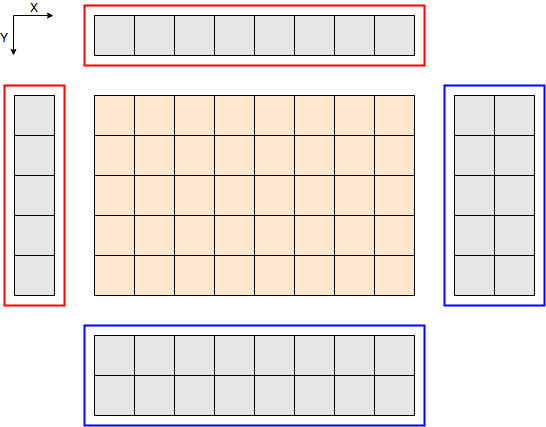
\includegraphics[width=0.9\linewidth]{2D_Block.png}
  \caption{In the middle and in light red the grid points belonging to this subdivision.
Outside in gray the four halo regions.
The red and blue lines surrounding the halo region indicates negative and positive directions respectively.}
  \label{fig:2DBlock}
\end{subfigure}%
\begin{subfigure}{0.2\textwidth}
  \centering
  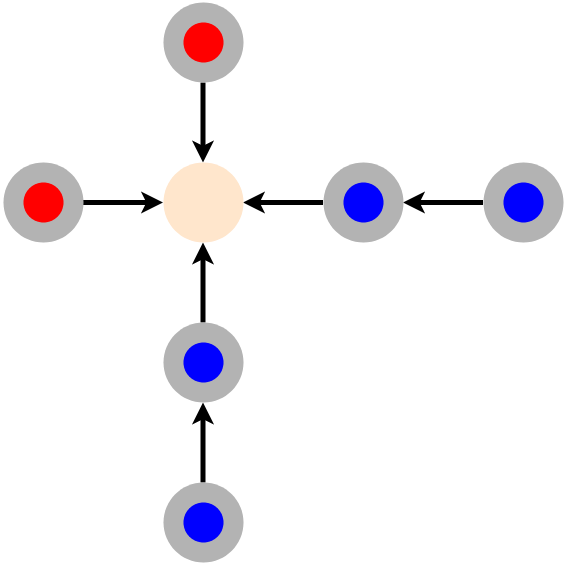
\includegraphics[width=0.9\linewidth]{2D_Block_stencil.png}
  \caption{Stencil representation corresponding to the subdivision on the left panel.}
  \label{fig:2DBlockStencil}
\end{subfigure}
\caption{Schematic view of a single two-dimensional domain subdivision.}
\label{fig:2D_subdivision}
\end{figure}

\begin{figure}[!htbp]
\centering
\begin{subfigure}{0.8\textwidth}
  \centering
  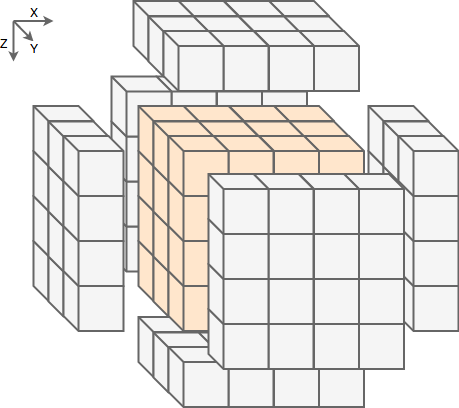
\includegraphics[width=0.9\linewidth]{3D_Block.png}
  \caption{In the middle and in light red the grid points belonging to this subdivision.
Outside in gray the six halo regions.}
  \label{fig:3DBlock}
\end{subfigure}%
\begin{subfigure}{0.2\textwidth}
  \centering
  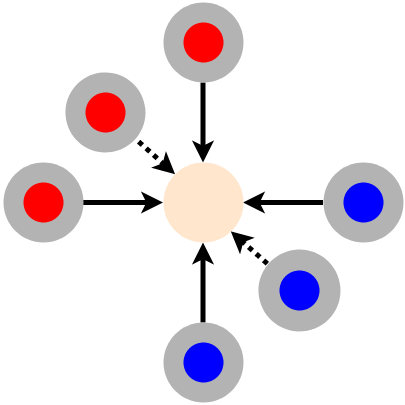
\includegraphics[width=0.9\linewidth]{3D_Block_stencil.png}
  \caption{Stencil representation corresponding to the subdivision in figure \ref{fig:3DBlock}.}
  \label{fig:3DBlockStencil}
\end{subfigure}
\caption{Schematic view of a single three-dimensional domain subdivision.}
\label{fig:3D_subdivision}
\end{figure}

\subsubsection{Source graph generation}
\label{sec:sourcegraphgeneration}
With the subdivision model definition and the two cost functions defined the source graph can be easily generated.
As shown in lines 14 to 20 of Algorithm \ref{alg:domaindecomposition} the source graph is generated as a weighted adjacency list by iterating over all subdivisions to determine their neighbors and handle the physical domain boundaries.

Determining the neighbors is an uncomplicated index calculation, as shown in Eq. \ref{eq:index} and handling the physical domain boundaries only requires catching the corresponding cases during the index calculation.

\begin{equation}
neighborindex = \left(\left(i + x\right) \cdot ndy + \left(j + y\right)\right) \cdot ndz + \left(k + z\right) \text{ ,}
\label{eq:index}
\end{equation}
where $i, j, k$ are the index number of the current subdivision in each dimension, and $x, y, z$ are either $-1$ for the negative neighbor in the corresponding direction, $+1$ for the positive neighbor in the direction, and $0$ otherwise. 
Also, $ndy, ndz$ are the number of subdivisions in y-direction and z-direction respectively.

The weighted adjacency list consists of four arrays.
The array $vweights$ contains the vertex weight for each subdivision i.e. vertex, thus its length is equal to the total number of subdivisions.
The array $eweights$ similarly contains the edge weight for each edge, and is therefore twice as long as the number of edges.
The array $adjncy$ contains the index of the end vertex for each edge, and is therefore twice as long as the number of edges.
The order in $adjcny$ determines the starting vertex for each edge.
It starts with the edges of the vertex with index 0, after all edges of vertex 0 it continues with edges of vertex 1 and so on.
And lastly the array $xadj$ contains for each vertex the $adjncy$-index for the first edge that does not belong to the vertex.
The array $xadj$ has the length of the total number of subdivisions.

The two arrays containing information about the edges are twice as long as the number of edges since graph partitioning methods do not require undirected graphs, even though for domain decomposition only undirected graphs are used.

An example adjacency list in this format can be seen in fig. \ref{fig:adjacency}, this adjacency list is the one corresponding to the source graph used in fig. \ref{fig:sourcegraph}.

\begin{figure}[!htbp]
  \centering
  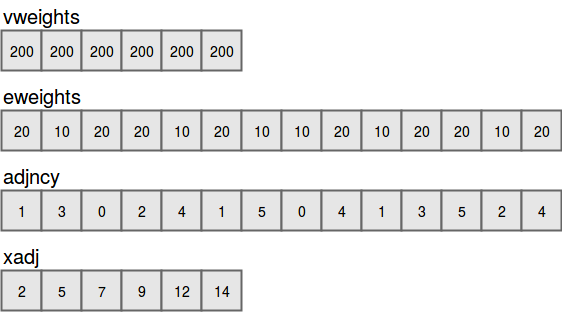
\includegraphics[width=0.8\linewidth]{adjacency.png}
  \caption{Weighted adjacency list arrays for source graph in the left panel.}
  \label{fig:adjacency}
\end{figure}

\subsection{Load balancing - graph partitioning method}
Once a domain is over-decomposed and the model has used its communication and computational cost estimates to generate a source graph the graph partitioning algorithm can be used to distribute the subdivisions into one partition for each processing unit.

Graph partitioning on such a weighted source graph means cutting the graph into partitions such that the edge cut between all partitions is minimized (i.e. minimal communication cost) while also keeping the vertex weights balanced (e.g. balanced computational cost).

More details about the graph partitioning method can be found in \citet{karypis1998multilevel} and are not the focus of this thesis.

The output of the graph partitioning methods is a list of indices for each vertex i.e. subdivision the index corresponds to a partition i.e. the index of a processing unit.

\paragraph{A small example}to demonstrate a few of the key characteristics of graph partitioning is shown in Fig. \ref{fig:sourcegraph}.
Specifically, Fig. \ref{fig:sourcegraph} shows three possible partitions for an example source graph.
For visual simplicity a two-dimensional domain is used, however a three-dimensional domain would work in the same way.
The source graph corresponds to a domain of size $30 \times 40$ with three subdivisions in x-direction and two subdivisions in y-direction.
In this example these six subdivisions are partitioned into two partitions, represented by the color of the circle in the Fig. \ref{fig:cut1}, Fig. \ref{fig:cut2}, and Fig. \ref{fig:cut3}.

Figure \ref{fig:cut1} shows a case where a graph partitioning cut causes a computational imbalance between the partitions.
Partitioning one subdivision more to one partition in such a small example causes a very large imbalance.
Usually the graph partitioning method would not allow a result with this much imbalance.
However, in larger graphs some computational imbalance up to a threshold is very common.
Most graph partitioning methods allow manipulating the imbalance threshold.

The mixed direction cut shown in Fig. \ref{fig:cut2} has the largest communication cost of the three partitions shown here.
However, it is a fully valid partition and partition boundaries that look similar are common in partitioning of larger graphs.
See the boundary between the brown and red partition in Fig. \ref{fig:metis1} for example.
This should highlight the importance of having defined clear and simple defined boundaries in the subdivision model, since the graph partitioning model already adds complexity to the partition boundaries.

Finally, Fig. \ref{fig:cut3} shows the ideal case for this small example.
Ideal cuts like this are only likely in such small and simple cases.

\begin{figure}[!htbp]
\centering
\begin{subfigure}{0.43\textwidth}
  \centering
  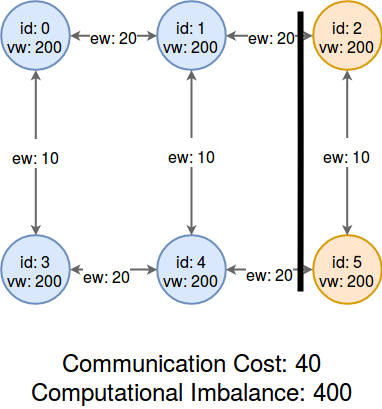
\includegraphics[width=0.95\linewidth]{source_graph_cut3.png}
  \caption{X-direction cut.}
  \label{fig:cut1}
\end{subfigure}%

\begin{subfigure}{0.43\textwidth}
  \centering
  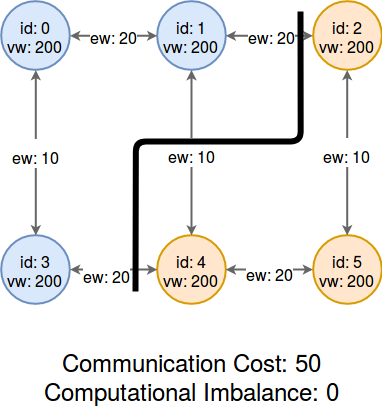
\includegraphics[width=0.95\linewidth]{source_graph_cut2.png}
  \caption{Mixed direction cut.}
  \label{fig:cut2}
\end{subfigure}%

\begin{subfigure}{0.43\textwidth}
  \centering
  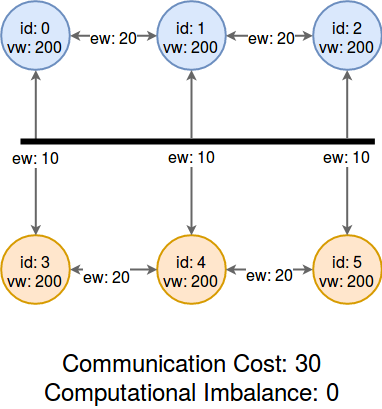
\includegraphics[width=0.95\linewidth]{source_graph_cut1.png}
  \caption{Y-direction cut.}
  \label{fig:cut3}
\end{subfigure}\hfill
\caption{Visual representation for a small graph partitioning example.
Each circle represents one subdivision of size $10 \times 20$.
The label "id" is the subdivision identification number.
The label "vw" describes the vertex weight and is equal to the size of the subdivision.
The label "ew" describes the edge weight and is equal to the size of the boundary between the corresponding subdivisions.
The color of the circle depicts the corresponding partition.
The thick, black line shows the boundary between the two partitions i.e. the cut chosen by the graph partitioning.}
\label{fig:sourcegraph}
\end{figure}

\subsection{Example subdivision and domain decomposition}
\label{sec:examplesubdivision}
The following example should highlight some aspects of the discussed subdivision and domain decomposition.

All the following figures in this section use the same domain and stencil.
The domain has size $2048 \times 1024 \times 40$ and the stencil extents are given as $\left[1, 1, 1, 1, 0, 0\right]$.
This means the stencil uses $1$ neighboring grid point in negative and positive x- and y-direction.
The boundary of the domain is also periodic in x-direction and non-periodic in y- and z- direction.

Figures \ref{fig:metis1}, \ref{fig:pymetis1}, and \ref{fig:scotch1} show the results if the domain is split into $16 \times 8 \times 1$ subdivisions.
This means every box in the figures represents $128 \times 128 \times 40$ grid points.

For comparison Figs. \ref{fig:metis2}, \ref{fig:pymetis2}, and \ref{fig:scotch2} show the results if the domain is split into $32 \times 16 \times 1$ subdivisions.
This means every box in the figures represents $32 \times 32 \times 40$ grid points and 4 of these boxes correspond to one box in the figures on the left side.

This comparison should highlight the difference the number of subdivisions and their size can make for the overall domain decomposition.
Also the difference the graph partitioning can make is shown in Fig. \ref{fig:rectangular1}.


\begin{figure}[!htbp]
\centering
\begin{subfigure}{0.5\textwidth}
  \centering
  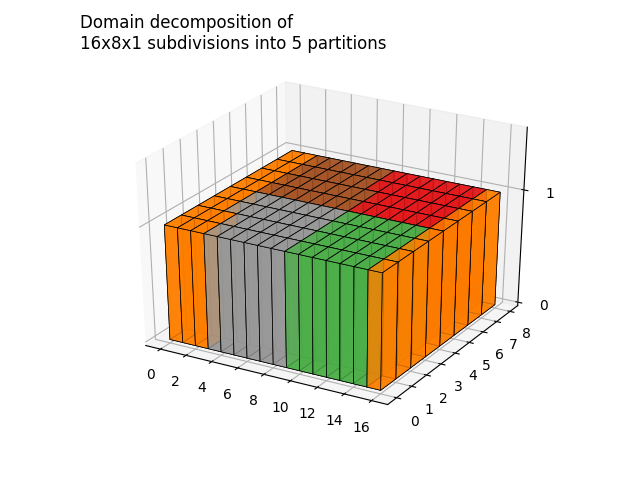
\includegraphics[width=0.9\linewidth]{metis16Px8x1.png}
  \caption{Partitioned by Metis.}
  \label{fig:metis1}
\end{subfigure}%
\begin{subfigure}{0.5\textwidth}
  \centering
  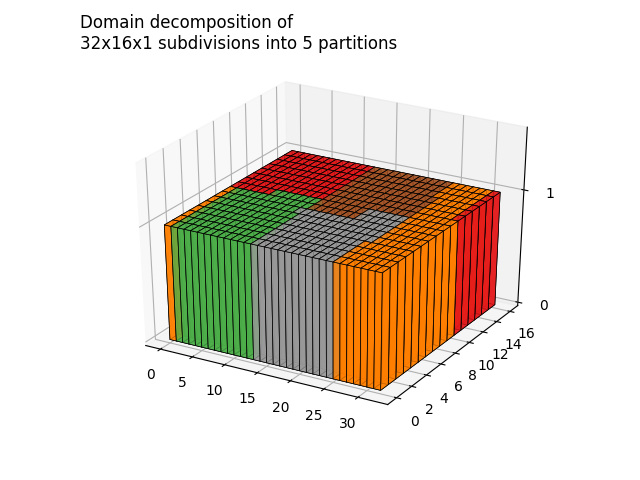
\includegraphics[width=0.9\linewidth]{metis32Px16x1.png}
  \caption{Partitioned by Metis.}
  \label{fig:metis2}
\end{subfigure}

\begin{subfigure}{0.5\textwidth}
  \centering
  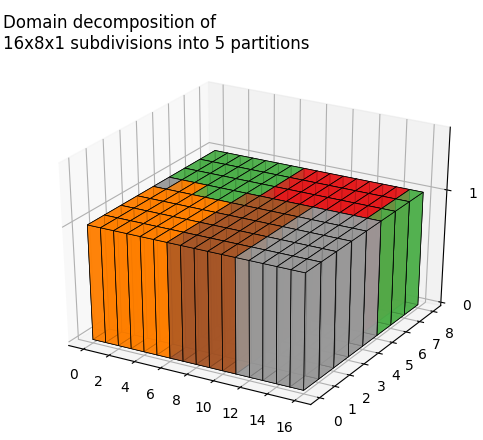
\includegraphics[width=0.9\linewidth]{pymetis16Px8x1.png}
  \caption{Partitioned by PyMetis}
  \label{fig:pymetis1}
\end{subfigure}%
\begin{subfigure}{0.5\textwidth}
  \centering
  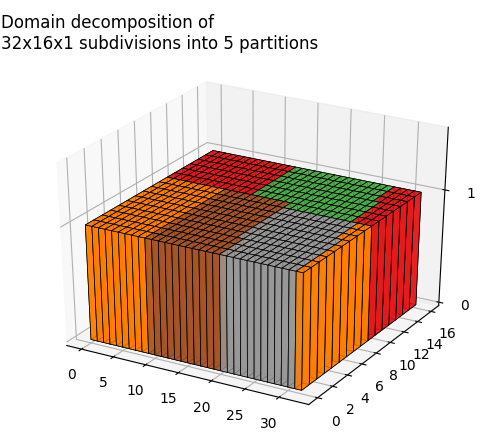
\includegraphics[width=0.9\linewidth]{pymetis32Px16x1.png}
  \caption{Partitioned by PyMetis}
  \label{fig:pymetis2}
\end{subfigure}

\begin{subfigure}{0.5\textwidth}
  \centering
  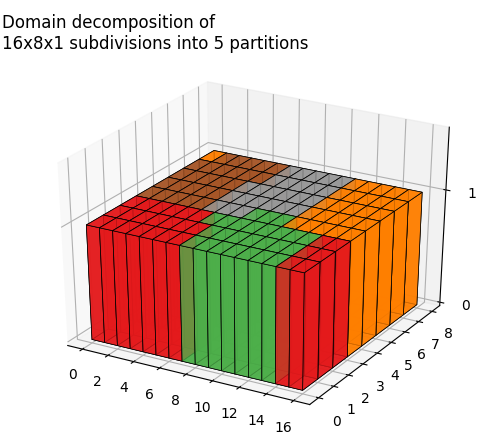
\includegraphics[width=0.9\linewidth]{scotch16Px8x1.png}
  \caption{Partitioned by Scotch}
  \label{fig:scotch1}
\end{subfigure}%
\begin{subfigure}{0.5\textwidth}
  \centering
  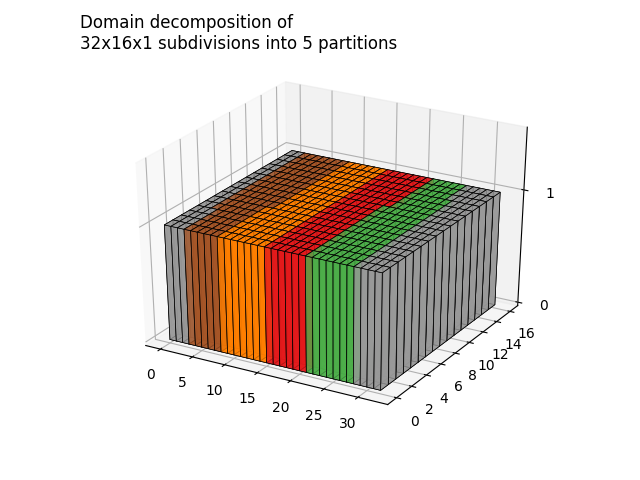
\includegraphics[width=0.9\linewidth]{scotch32Px16x1.png}
  \caption{Partitioned by Scotch}
  \label{fig:scotch2}
\end{subfigure}

\caption{Domain subdivision and domain decomposition into 5 partitions. 
Each box represents one subdivision of grid points.
Each color represents one partition. 
The domain has size 2048 x 1024 x 40 and a periodic boundary in x-direction.
Even though the domain is fully three dimensional, the domain is only decomposed in the x-y plane i.e. the horizontal plane.
Such a decomposition represents an often encountered use case for domains where the size of the two horizontal dimensions are much larger than the size of the vertical dimension e.g. numerical weather prediction models.
Not decomposing in the vertical dimension is important for locality and performance since the vertical dimension is usually the innermost loop dimension.
This also fits with many parameterizations that use the single column model assumption.
}
\label{fig:rectangular1}
\end{figure}


\section{Library design and implementation}

\section{Case study}

To show the functionality and applicability of the automatic domain decomposition library a few case studies were carried out.
This chapter and the following sections will outline each case study and the corresponding experimental results.

\subsection{Case 1: Burger's equation}
Burger's equation is a well-known nonlinear partial differential equation.
It is widely used to test numerical schemes since it has analytical solutions for a set of initial conditions.
Burger's equation can be used to model various physical phenomena.
Most commonly it is used as a model for traffic flow or shock waves in a fluid.

\subsubsection{Case description}

The two-dimensional, viscid Burger's equation is given by the following system of equations as described in \citet{zhao2011new}:

\begin{equation}
\begin{split}
\pdv{u}{t} + u \pdv{u}{x} + v \pdv{u}{y} = \epsilon \left( \pdv{^2 u}{x^2} + \pdv{^2 u}{y^2} \right) \\
\pdv{v}{t} + u \pdv{v}{x} + v \pdv{v}{y} = \epsilon \left( \pdv{^2 v}{x^2} + \pdv{^2 v}{y^2} \right) \\
\text{with } \left(x, y, t\right) \in D \cross \left(0,T\right]
\end{split}
\end{equation}

With the following set of initial and boundary conditions: 

\begin{equation}
\begin{split}
\text{Initial conditions: } \\
u\left(x, y, 0\right) = u_0\left(x, y\right), \left(x, y\right) \in D \\
v\left(x, y, 0\right) = u_0\left(x, y\right), \left(x, y\right) \in D \\
\text{Boundary conditions: } \\
u\left(x, y, t\right) = f\left(x, y, t\right), \left(x, y, t\right) \in \partial D \cross \left(0, T\right] \\
v\left(x, y, t\right) = g\left(x, y, t\right), \left(x, y, t\right) \in \partial D \cross \left(0, T\right]
\end{split}
\end{equation}

The first set of initial and boundary conditions are the ones used by Shankar. \footnote{https://ch.mathworks.com/matlabcentral/fileexchange/38087-burgers-equation-in-1d-and-2d}

The second set of initial and boundary conditions are the same as used in \citet{zhao2011new}:

\subsubsection{Implementation details}

\subsubsection{Experimental setup}

\subsubsection{Experimental results}


\subsection{Case 2: Shallow water equation}

\subsubsection{Case description}

\subsubsection{Implementation details}

\subsubsection{Experimental setup}

\subsubsection{Experimental results}

\section{Conclusion}



\newpage
% === Bibliography ===
\bibliographystyle{plainnat}
\bibliography{bibl_conf}


% === Appendices ===
\pagebreak
\section{Appendix}
The appendix contains:
\begin{itemize}
%\item Full results for the scaling study on the Greina nodes.
\item Declaration of originality
\end{itemize}
\renewcommand{\thesubsection}{\Alph{subsection}}
\section*{Appendix}

%\subsection{Full results for the scaling study on the Greina nodes.}
%%\includepdf[pages={-}]{Scaling_Results_Greina_Nodes.pdf}
%\noindent
%\includegraphics[
%    page=1,
%    width=1.3\textwidth,
%    height=1.3\textheight,
%    keepaspectratio
%]{Scaling_Results_Greina_Nodes.pdf}
%\vfill

\subsection{Declaration of originality}
%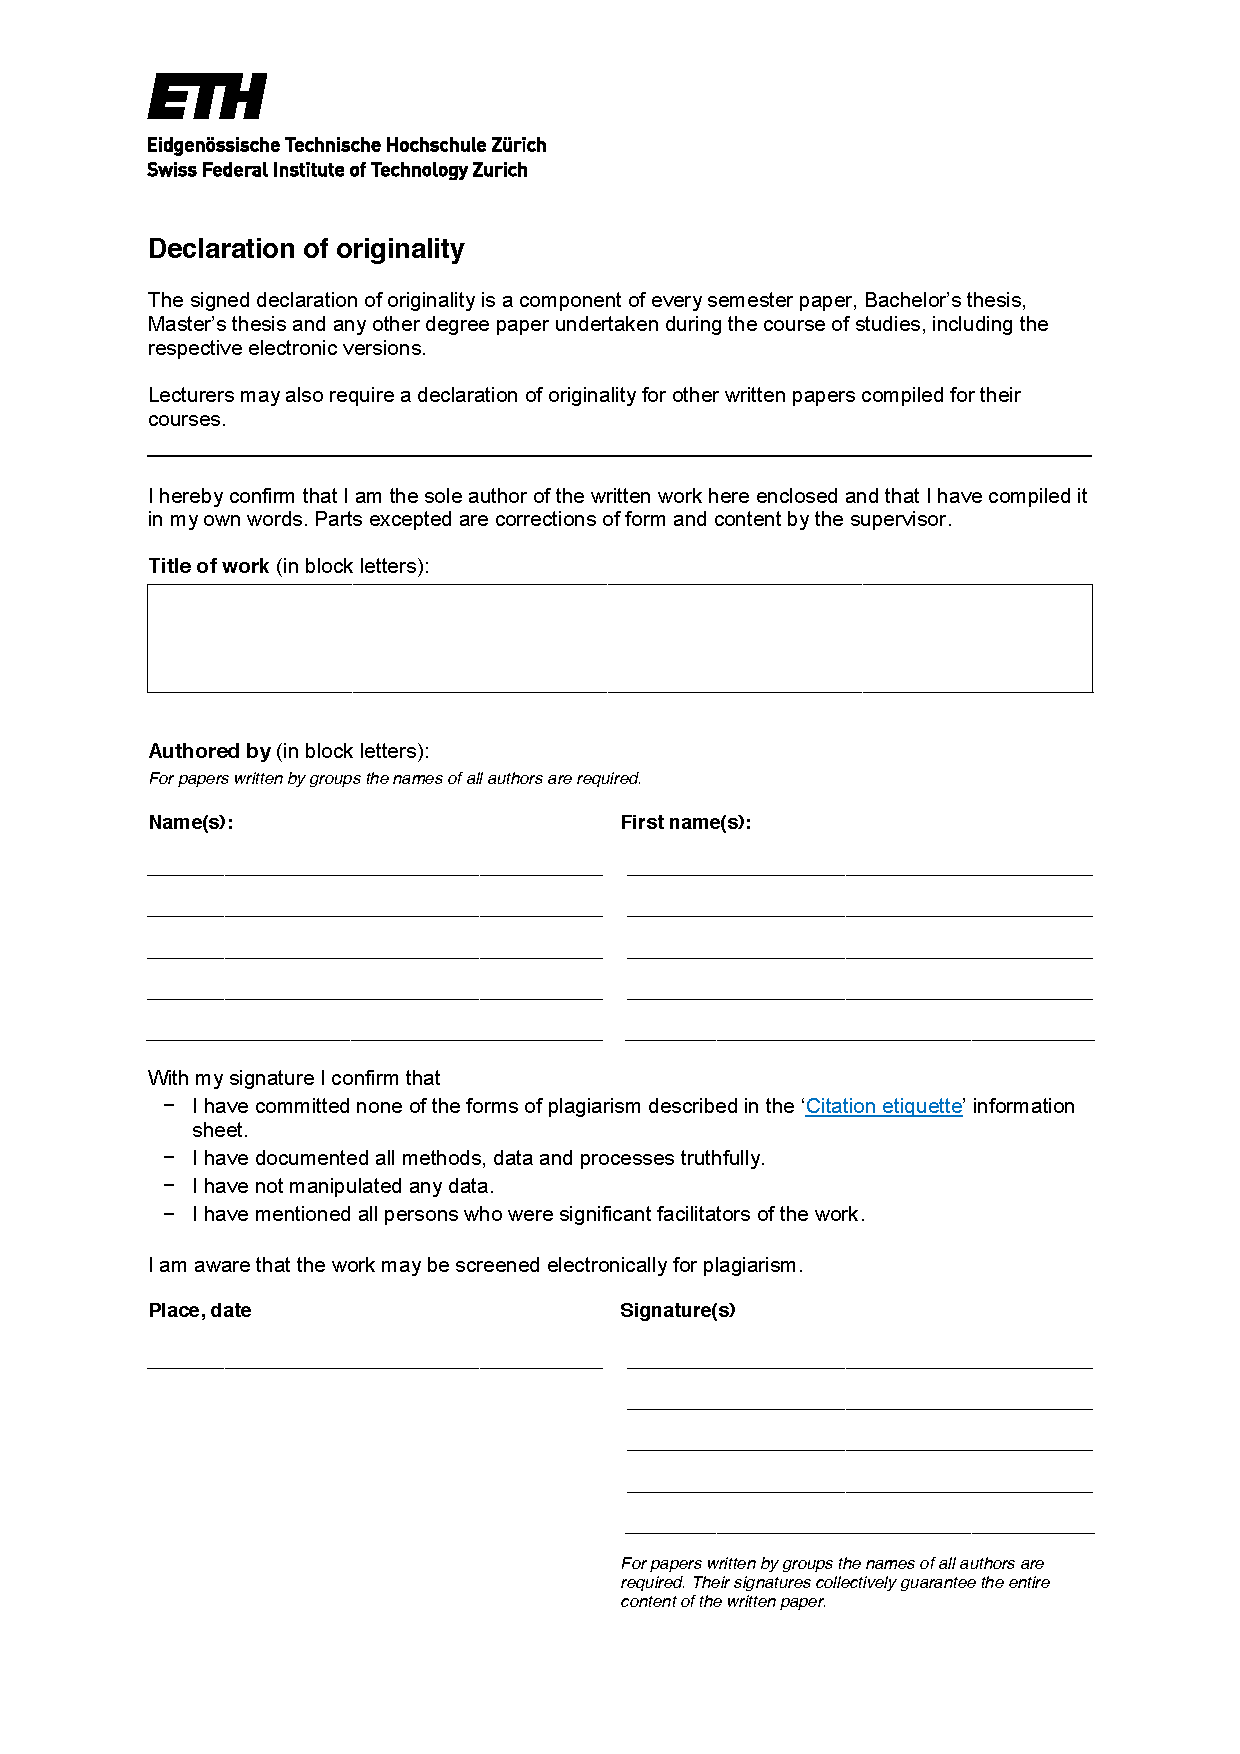
\includepdf[pages={-}]{declaration-originality.pdf}
\noindent
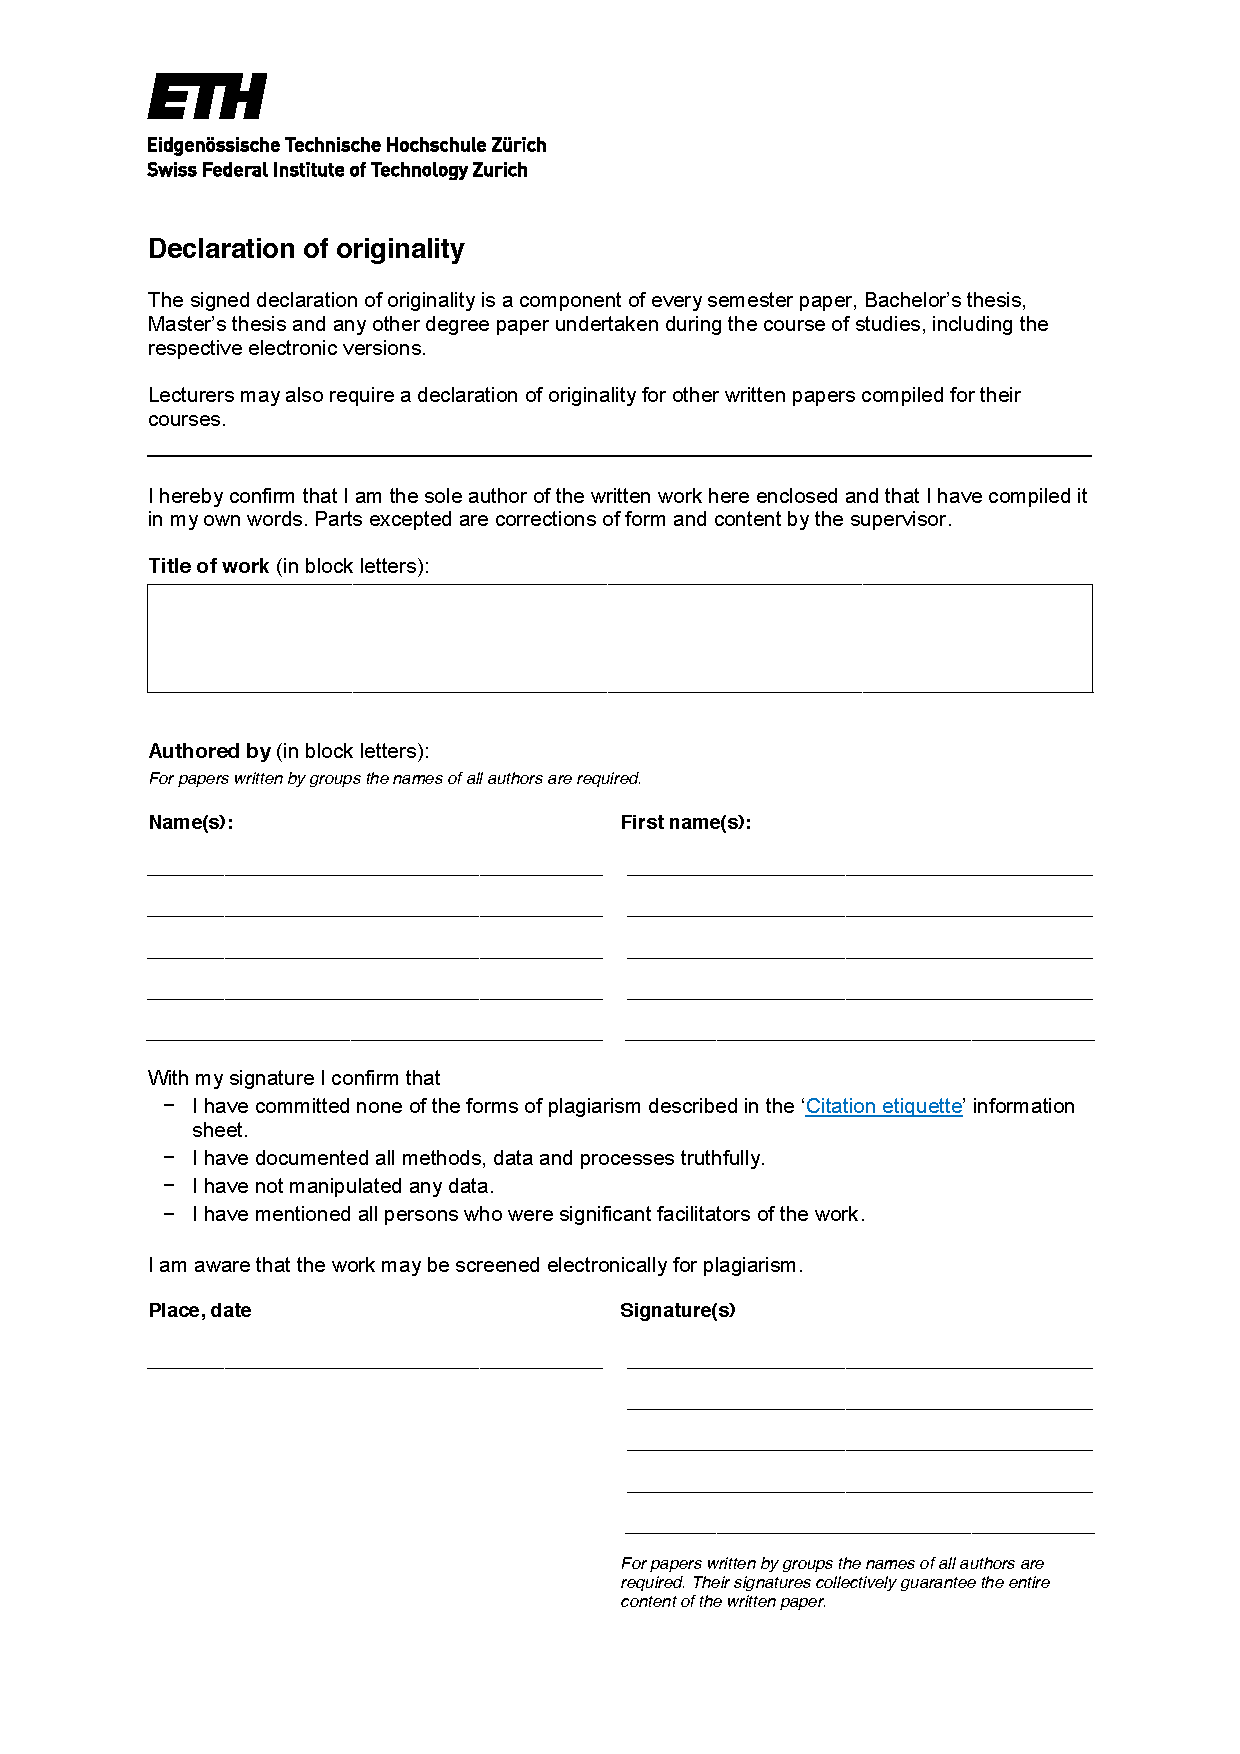
\includegraphics[
    page=1,
    width=1.2\textwidth,
    height=1.2\textheight,
    keepaspectratio
]{declaration-originality.pdf}
\vfill


\end{document}
